\documentclass{book}
\usepackage{hyperref}
\usepackage{graphicx}


\title{Documentazione}
\author{Benedetta Vitale - Emilio Meroni}
\date{18 Novembre, 2023}

\graphicspath{{../../Immagini}}

\begin{document}

\maketitle

\tableofcontents    

\chapter{Project Plane}

\section{Introduzione}

Questo progetto verrà svolto da Benedetta Vitale ed Emilio Meroni, 
entrambi studenti al terzo anno di ingegneria informatica presso 
l'università di Bergamo.

Il software che andremo a sviluppare è pensato per dare supporto 
alla attività di ristorazione. In particolare, dovrà assistere alle mansioni dei camerieri, come, prendere le ordinazioni ai tavoli, redigere il conto, trovare tavoli disponibili, ecc.

Abbiamo scelto questa tipologia di sistema dato che Emilio lavora, nei week-end, presso un ristorante, e gli ha incuriosito la gestione interna tramite l'utilizzo dei palmari da parte dei camerieri. 

\section{Modello di Processo}

Il modello di processo che seguiremo è quello della prototipazione, in particolare la prototipazione evolutiva [Figura: \ref{fig: modello_processo_evolutivo}], molto utile per quanto riguarda la costruzione dell'interfaccia grafica, la parte principale della nostra applicazione.

\begin{figure}
    \centering
    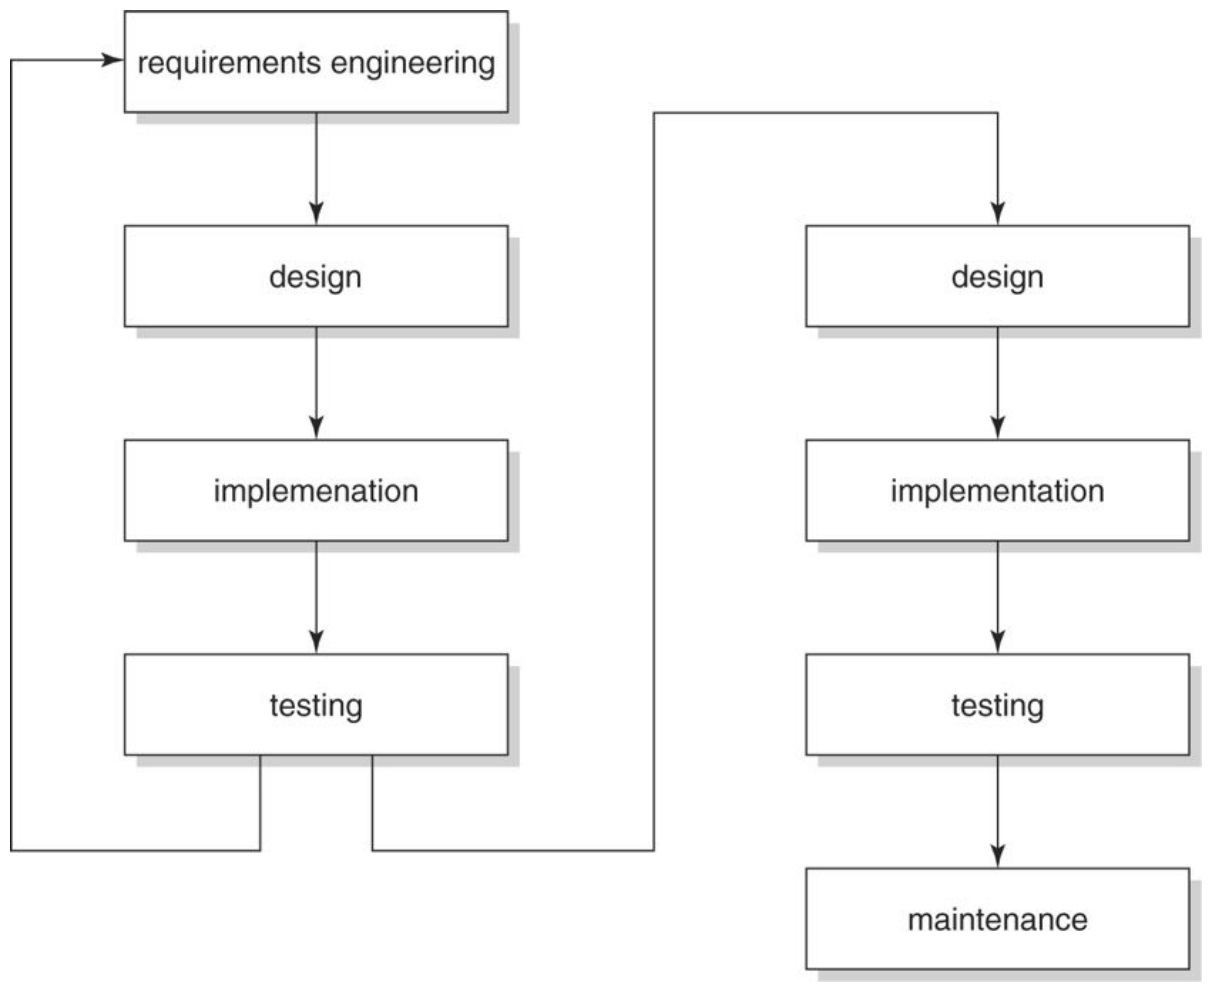
\includegraphics[width = 0.7\linewidth]{../../Immagini/Modello_Processo_Evolutivo.jpg}
    \caption{Modello Di Processo Evolutivo}
    \label{fig: modello_processo_evolutivo}
    
\end{figure}

\section{Organizzazione del Progetto}

Utilizzeremo una organizzazione a tre livelli:

\begin{enumerate}
    \item Livello Data Base
    \item Livello Logico
    \item Livello Presentazione
\end{enumerate}
Il \textit{livello Data Base}, come da nome, si occuperà della parte del DB, il quale sarà embedded, SQLite.
Il \textit{livello Presentazione} sarà quello visto dall'utente che usufruirà dell'applicazione, possiamo definirlo come il livello più esterno dove i dati verranno presentati in modo grafico e la gestione dei tavoli e delle comande è fatto in modo interattivo.
L'ultimo livello è quello \textit{Logico}, il quale possiamo posizionarlo graficamente tra il livello Data Base e quello Presentazione, funge da intermediario tra i due livelli e fornisce gli oggetti principali per la gestione dell'applicazione


\section{Standard, Lineeguida, Procedure}

Per la parte della stesura della documentazione si è scelto di utilizzare uno tool molto utile nella stesura di documenti professionali, \textit{laTeX}. scelta quasi obbligata derivata dall'utilizzo di \textit{GitHub} insieme al programma di scrittura precendente \textit{Microsoft Word} il quale ha causato difficolta nei "merge" su \textit{GitHub}.

 mentre per la parte di \textit{codifica} abbiamo scelto di utilizzare lo standard definito da \textit{Java}\footnote{Standard di Java si possono trovare su questo \href{https://www.oracle.com/java/technologies/javase/codeconventions-contents.html}{\underline{sito}}}, in primo luogo perché l'IDE utilizzato per la parte di progammazione è \textit{Eclipse} il quale fornise strumenti per la formatttazione e nominazione di metodi in modo automatico secondo gli standard di \textit{Java}, inoltre, non avendo entrambi molta esperienza ci è venuto comodo utilizzare uno dei pochi standard di codificha che conosciamo.

 Lo strumento che utilizzeremo per la condivisione della documentazione e del codice sarà, come già anticipato, la piattaforma di condivisione \textit{GitHub}.
\section{Attività di Gestione}


\section{Rischi}

In questa sezione si discutono i rischi che potrebbero verificarsi durante lo sviluppo progetto. 

Un primo rischio evidenzianto da entrambe le parti sono le difficoltà che potrebbero verificarsi nell'utilizzo di \textit{windows builder}, plugin che consente la progettazione visuale dell'interfaccia utente su \textit{Eclipse}, dovuta da una bassa conoscenza del tool. Un probabile "effetto" sarà quello di allungare i tempi di codifica sul modulo di presentazione.

\section{Personale}
Il numero di persone che lavoreranno a questo progetto sarà molto ristretto, nello specifico sono: 
\begin{itemize}
    \item Benedetta Vitale
    \item Emilio Meroni
\end{itemize}
I quali participeranno in modo equo a tutte le attività, sia in scrittura della documentazione che sulla parte di codifica. Si è deciso che si lavorerà spesso in coppia, in particolar modo sulla parte di programmazione dato che la parte grafica su \textit{Java} non è mai stata approfondita da entrambe le parti e questo progetto ne ha una parte molto importante.
     

\section{Metodi e Tecniche}



\section{Garanzia e Qualità}

Il programma dovrà essere utilizzato in ristoranti, e in particolare dal personale che prenderà le ordinazioni, quindi dovrà essere di \textit{facile} utilizzo, con un focus maggiore sulla funzionalità che sull'estetica. Un'altra qualità che dovrà garantire è la \textit{prevenzione di errori} da parte degli utenti, come ad esempio il "miss-click" (click errati o accidentali).
In particolare abbiamo evidenziato quattro qualità che il sistema dovrà possedere:

\begin{enumerate}
    \item \textbf{Semplice}: Il programma sarà scritto per avere poche sezioni scritte e di facile comprensione, anche per chi si approcia al programma per la prima volta. Si utilizzeranno poche schermate che contengono tutto il necessario per le \textit{macro} operazioni definite nelle specifiche dei requisiti e indicate nel case diagram [Figura: \ref{fig: use_case_diagram}].
    \item \textbf{Intuiblile}: L'utilizzo dei colori per indicare gli stati dei \textit{tavoli}, in particolre si è deciso che per i \textit{tavoli liberi} si utilizzara il colore verde, per i \textit{tavoli occupati} il colore rosso e per i \textit{tavoli da pulire} l'arancione [Figura: \ref{fig: es_bottoni}].
    \item \textbf{Prevenzione Errori}: Per la prevenzione degli errori si utilizzeranno schermate \textit{pop-up}, per la convalida degli input
    \item \textbf{Veloce}: Con questo termine si indica che il programma, che verrà utilizzato da dispositivi touch, dovrà essere principalmente composto da bottoni che minimizzano i tempi di utilizzo, puntando a un uso minimo della tastiera. Comportando un'esperienza più agevole per l'utente.
\end{enumerate}

\begin{figure}[h]
    \centering
    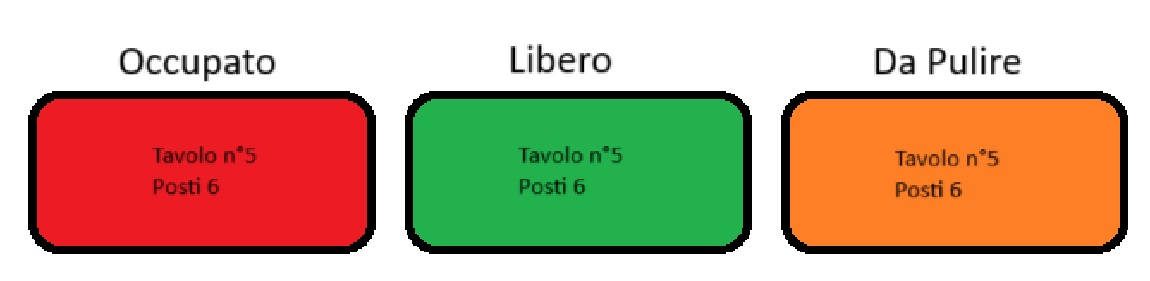
\includegraphics[width=0.6\linewidth]{Esempio_Bottoni.jpg}
    \caption{Esempio di colorazione dei bottoni per i tavoli}
    \label{fig: es_bottoni}
\end{figure}


\section{Workpackages}

\section{Risorse}

Gli strumenti che verranno adottati in questo progetto saranno:
\begin{itemize}
    \item Per la parte di codifica, come già detto in precedenza, l'IDE \textit{Eclipse}, uno strumento specifico per la scrittura di codice e gestione di progetti \textit{Java}.
    \item In scrittura si utilizzerà l'editor di testo open source \textit{VS Code} con l'estensione \textit{LaTeX Workshop} per la scrittura di documenti in formato \textit{LaTeX}. Contribuendo garantire una presentazione accurata dei documenti.
    % \item Per la condivisione e gestione delle versioni del progetto intero (Strumenti di \textit{Software Configuration Management}) verrà impiegato il tool \textit{GitHub}.
    \item Infine, riguardo agli strumenti di \textit{Software Configuration Management}, adotteremo \textit{GitHub}. Questa piattaforma sarà impiegata principalmente per la condivisione, gestione e tracciamento delle modifiche al software, oltre che per la documentazione. 

\end{itemize}

\section{Budget}

Per quanto riguarda il budget, si è previsto un tempo totale di 80 ore lavorative. con una forte attenzione sulla parte di documentazione rispetto a quella di codice.
In prima approssimazione possiamo definire una divisione del tempo come mostrato in figura [\ref{fig: diagramma_gant}]. 
\begin{figure}[h]
    \centering
    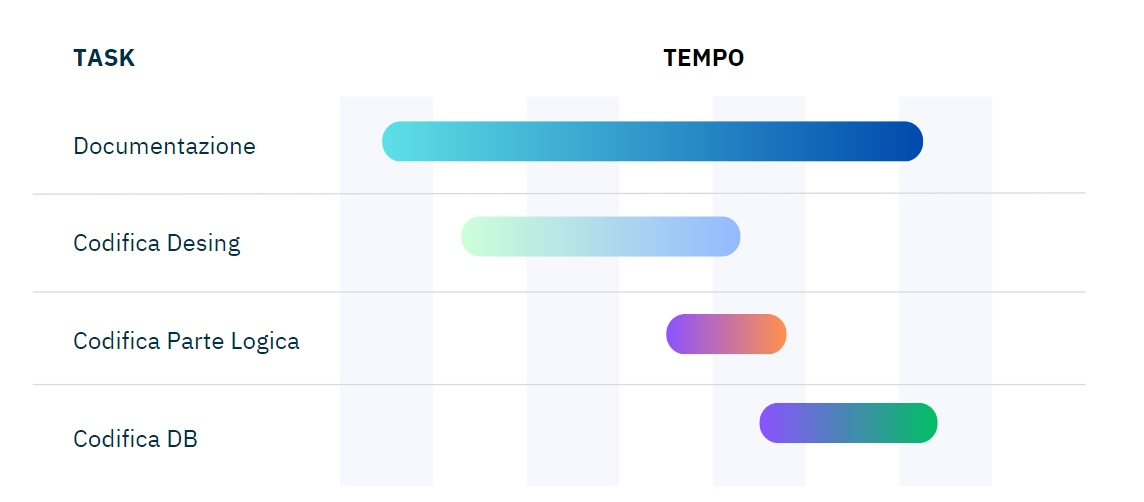
\includegraphics[width = 1\linewidth]{Diagramma_Gant.jpg}
    \caption{Diaramma di Gant}
    \label{fig: diagramma_gant}    
\end{figure}

\section{Cambiamenti}

% dichiarare come verranno gestite le modifiche proposte

\section{Consegna}


In questa sezione si discutono i metodi e le scadenze di consegna del progetto, in particolare la consegna si dividerà in due fasi:


\begin{itemize}
    \item Consegna del \textit{Project Plane}, il quale dovrà essere consegnato circa un mese prima del primo esame scritto, che si svolgerà nel mese di gennaio; quindi, per il mese di dicembre si dovrà effettuare la prima consegna.
    \item Consegna del \textit{Progetto}, quest'ultimo avrà una scadenza più lunga, infatti, l'ultimo giorno di consegna sarà cinque giorni prima dell'esame orale.
\end{itemize}
Per quanto riguarda i metodi di consegna si dovrà condividere con il professore Gargantini la repository di github contenente il progetto, per la consegna di questo documento si dovrà indicare nel file reame, della repository, la posizione del project plane. Mentre per la consegna del progetto si dovrà creare un \textit{issue}, intitolata “Approvazione Progetto” ed assegnarla al professore.

\chapter{Specifiche dei Requisiti}

\begin{figure}[ht]
    \centering
    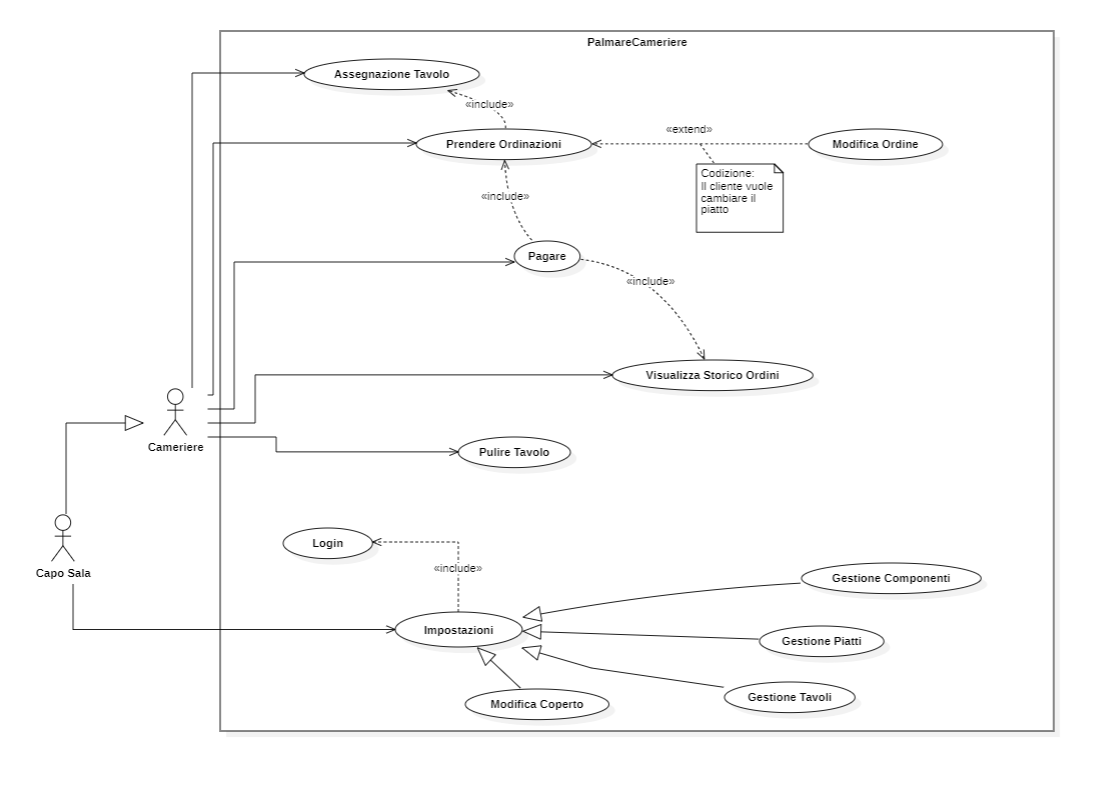
\includegraphics[width=1\linewidth]{../../UML/Diagrammi/Use_Case_Diagram.png}
    \caption{Use Case Diagram}
    \label{fig: use_case_diagram}
\end{figure}

\end{document}